\documentclass[12pt, a4paper]{article}
\usepackage{fontenc}
\usepackage{graphicx}
\usepackage{amsmath}
\graphicspath{ {./images/} }
\usepackage[ddmmyyyy]{datetime}
\usepackage{pdflscape}

\renewcommand{\dateseparator}{.}
\renewcommand{\contentsname}{İçindekiler}
\renewcommand{\figurename}{Şekil}
\renewcommand{\refname}{Kaynakça}


\title{\textbf{Yapay Zeka Tabanlı Ses Üretimi}\large }
\author{\textbf{Beyzanur Dağdelen}\large}
\date{\textbf{\today}}

\makeatletter         
\def\@maketitle{
	\textbf{\large{KÜTAHYA SAĞLIK BİLİMLERİ ÜNİVERSİTESİ}\centering}\\[4ex]
	\centering
	
\includegraphics[width = 40mm]{ksbu.png}\\[8ex]
	\begin{center}
		{\large \bfseries \@title }\\[4ex] %\Huge
		{\small  \@author}\\[4ex] 
	
		\vspace{10\baselineskip}
		{\large \bfseries \subitem}
		\section*{\centering Danışman}
		\section*{\small \centering Dr.Öğr.Üyesi Emre Güngör}
		\section*{\small Yapay Zeka \& Veri Odaklı Sistem Tasarımı \& Latex İle Rapor Hazırlama}
		\vspace{2\baselineskip}
		\@date 
\end{center}}
\makeatother


\begin{document}
	
	\maketitle
	
	\thispagestyle{empty}
	
	\newpage
	\tableofcontents  %içindekiler
	\pagenumbering{arabic}
	\newpage

	\section{Giriş} 	\vspace*{1\baselineskip}
	Bu proje, yapay zeka ile ses üretimine odaklanmaktadır. Günümüzde, yaşamdaki problemlerin sonucunda mutluluk, sevinç, heyecan gibi yaşamı olumlu etkileyen duyguların olduğu gibi stres, kaygı, korku, hayal kırıklığı gibi duygular da fazlasıyla yaşanmaktadır. Bu durum, insan yaşamını olumsuz etkileyebilmektedir. 
	 
	\raggedright Bu projenin amacı, iyileştirici etkiye sahip farklı frekanslardaki sesleri, yapay zeka ile üreterek insanlar üzerindeki olumsuz duygularını azaltarak, iyileştirmek ve motivasyon sağlayarak hayatlarındaki gelişen süreci desteklemektir.
	
	Frekansların iyileştirici etkisini desteklemek amacıyla unreal engine ortamındaki sanal gerçeklik teknolojisi ile  aynı zamanda insanı huzurlu hissettiren ortamlarda bu deneyimi sağlayarak rahatlama, stres azaltma ve motivasyon gibi faydalar sağlamayı amaçlamaktadır.
	\vspace*{3\baselineskip}
	
	\section{Literatür Taraması} 	\vspace*{1\baselineskip}
	Bu projede yapılan literatür taraması, frekansların iyileştiriciliği hakkında çalışmalar bulunmaktadır. 
	
	Farklı frekanslara maruz kalmak, depresyon veya anksiyete gibi psikiyatrik sorunları hafifletebilir ve aynı zamanda vücudu genetik sinyal yoluyla fiziksel rahatsızlıkları iyileştirmeye teşvik edebilir. Ünlü doktor, filozof, ve matematikçi Pisagor, frekansların vücut üzerinde iyileştirici bir etkiye sahip olduğuna ve günlük müziğe maruz kalmanın insan sağlığı için faydalı olduğuna ikna olmuştu. Pisagor, matematiksel oranlar ve farklı müzik akorları arasındaki harmonik ilişkiyi  keşfetmiştir\cite{myss2013anatomy}. 
	
	Randomize kontrollü bir çalışma olan Vasküler cerrahi popülasyonu için 22.5 kHz düşük frekanslı temas ultrason debridmanının (LFCUD) alt ekstremite yarası iyileşmesi üzerindeki etkisi için yapılan bu projenin amacı, düşük frekanslı temas ultrason debridmanı olan veya olmayan tedavi edilen vaskülopati ve düşük ekstremite yaraları olan hastalarda yara büyüklüğü ve görünüm ve sağlık komplikasyon oranlarındaki değişiklikleri karşılaştırmaktı (LFCUD) Bu çalışma randomize kontrollü bir çalışmadır. Çalışma, ayaktan yara kliniği ve yatan hasta koğuşu da dahil olmak üzere vasküler cerrahi hizmetinde, yükseköğretim akademik merkezinde gerçekleştirilmiştir. Toplamda, vaskülopati ve karışık etiyolojinin aşırı ekstremite yaraları olan 70 hasta çalışmaya dahil edildi; 68 çalışmayı tamamladı. Hastalar LFCUD artı olağan bakım almak üzere randomize edildi (n = 33) veya normal bakım (n = 37) haftalık 4 ziyarette ve daha sonra 12 hafta boyunca takip edildi. Ana sonuç ölçümleri, gözden geçirilmiş Fotoğrafik Yara Değerlendirme Aracı (revPWAT) tarafından kapalı yaralar, yara yüzey alanındaki değişiklik (WSA) ve yara görünümünü içermektedir. Haftalık 4 LFCUD tedavisinden sonra, LFCUD grubundaki hastalar, sadece normal bakımla tedavi edilen kontrol grubuna kıyasla önemli ölçüde daha iyi yara görünümüne sahipti .
	Bu çalışma sonucunda vasküler hastalık nedeniyle komplike olan yaraların iyileşme süreci daha uzun olduğu ve hastaların ciddi sağlık riskleriyle karşı karşıya kaldığı gözlemlenmiştir\cite{murphy2018effect}. 
	
	The Bioelectronic Basis for "Healing Energies" makalesinin yapıldığı tarih itibariyle, enerji parametrelerinin belirlendiği ve kontrol edildiği 150'den fazla "iyileştirici enerji" çalışması rapor edilmiştir\cite{roffey2012bioelectronic}.  
	\vspace*{2\baselineskip}
	
	\section{Metodoloji} 	  \vspace*{1\baselineskip}
	Yapay zeka algoritmaları ile istenilen frekanslarda sesler üretebilecek bir yapay zeka sistemi geliştirilecektir. Bu sistem keras,tensorflow gibi teknolojiler denenilerek tercihler sonucunda bu teknolojilerden yararlanılacaktır.
		
   	Unreal engine ortamında kullanıcıların sesleri ve 3 boyutlu ortamı deneyimleyebileceği bir sanal gerçeklik ortamı geliştirilecektir. 3D ortam tasarımı, sanal karakterler ve etkileşimli unsurlar bu aşamada oluşturulacak.Sanal gerçeklik deneyimi sahne ortamında test edilecektir.
	Unreal engine ortamında blueprint teknolojisi kullanılacaktır.
	
	\vspace*{1\baselineskip}	
	Bu projenin sanatsal vizyonuna ve sahne tasarımıma uygun assetler için unreal engine marketplaceden yararlanılmıştır.Görsel çeşitlilik ve ilgi çekici bir ortam yaratmak için gerçekçi assetler seçilmiştir.
	Sahneye renk ve canlılık katması için çiçekler, yapraklar ,farklı gökyüzü assetleri tercih edilmiştir.
	Deneyimleyenlere doğal ve huzurlu bir atmosfer yaratır.
	
	Aşağıdaki şekil \ref{Fig:Data1} , \ref{Fig:Data2}, \ref{Fig:Data3}, \ref{Fig:Data4} ,\ref{Fig:Data5} , \ref{Fig:Data6}, \ref{Fig:Data7}, \ref{Fig:Data8}'de görebileceği üzere
	gibi hazır assetler ile işlemler gerçekleştirilecektir. Doğanın ferahlatıcı dizaynı için kullanılabilecek bazı doğa assetleri aşağıdadır .
	
	\begin{figure}[!htb]
		\begin{minipage}{0.48\textwidth}
			\centering
			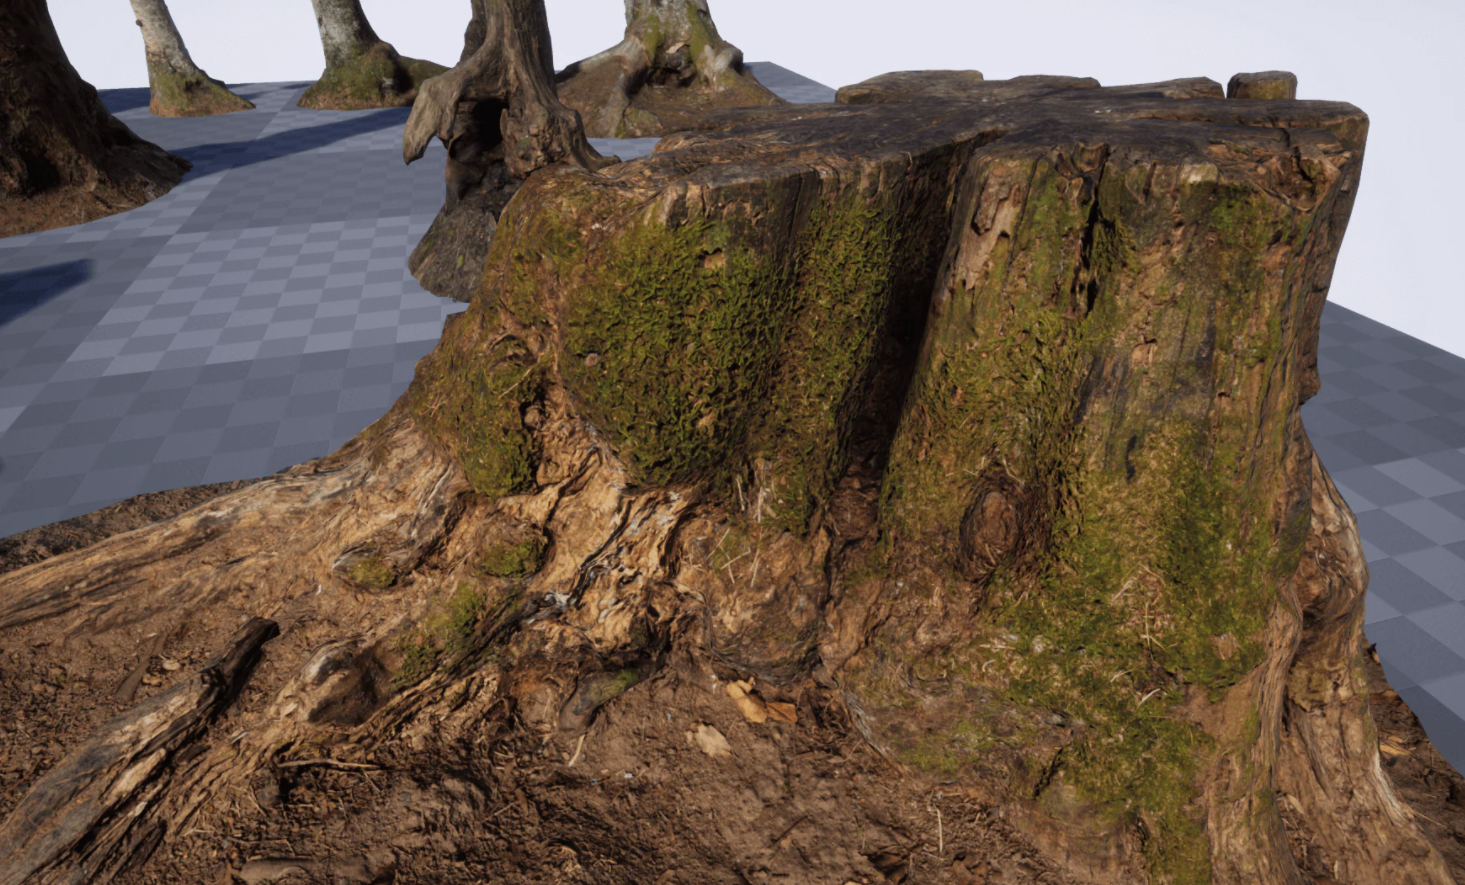
\includegraphics[width=.7\linewidth]{root.png}
			\caption{Kök}\label{Fig:Data1}
		\end{minipage}\hfill
		\begin{minipage}{0.48\textwidth}
			\centering
			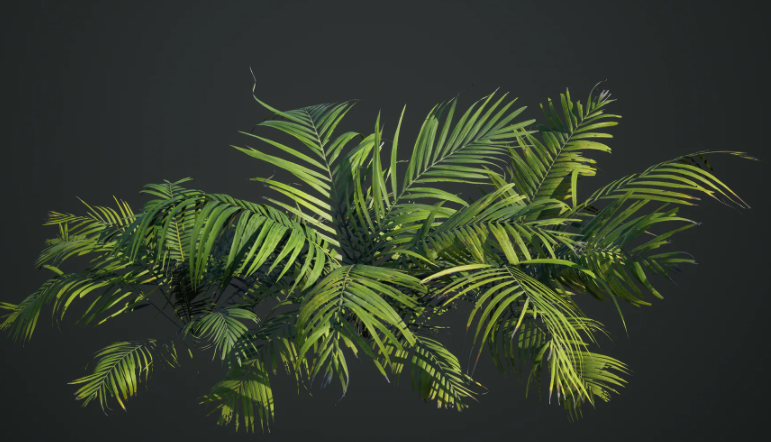
\includegraphics[width=.7\linewidth]{tropical.png}
			\caption{Bitki}\label{Fig:Data2}
		\end{minipage}
	\end{figure}
	
	\begin{figure}[!htb]
		\begin{minipage}{0.48\textwidth}
			\centering
			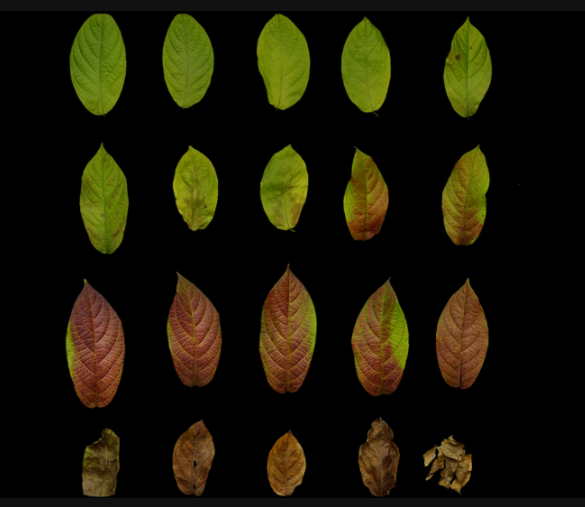
\includegraphics[width=.7\linewidth]{leaves.png}
			\caption{Yapraklar}\label{Fig:Data3}
		\end{minipage}\hfill
		\begin{minipage}{0.48\textwidth}
			\centering
			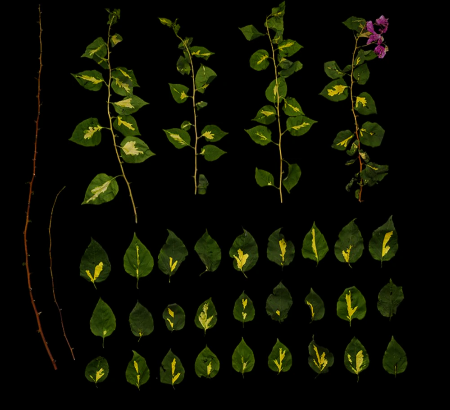
\includegraphics[width=.7\linewidth]{bush_leaf.png}
			\caption{Yapraklar}\label{Fig:Data4}
		\end{minipage}
	\end{figure}

	\begin{figure}[!ht]%b
		\begin{minipage}{0.48\textwidth}
			\centering
			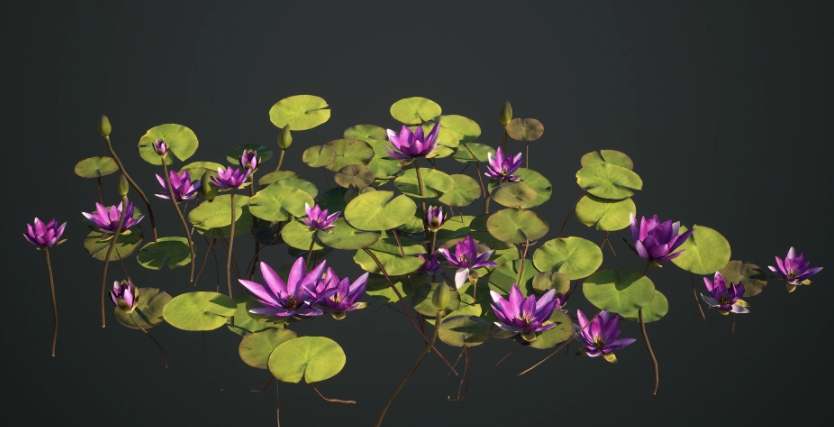
\includegraphics[width=45mm , height=48mm]{aquatic.png}
			\caption{Nilüfer}\label{Fig:Data5}
		\end{minipage}\hfill
		\begin{minipage}{0.48\textwidth}
			\centering
			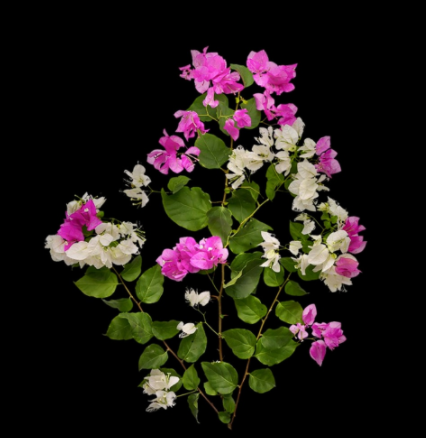
\includegraphics[width=.7\linewidth]{flower2.png}
			\caption{Çiçek}\label{Fig:Data6}
		\end{minipage}
	\end{figure}
	
		\begin{figure}[!ht]%b
		\begin{minipage}{0.48\textwidth}
			\centering
			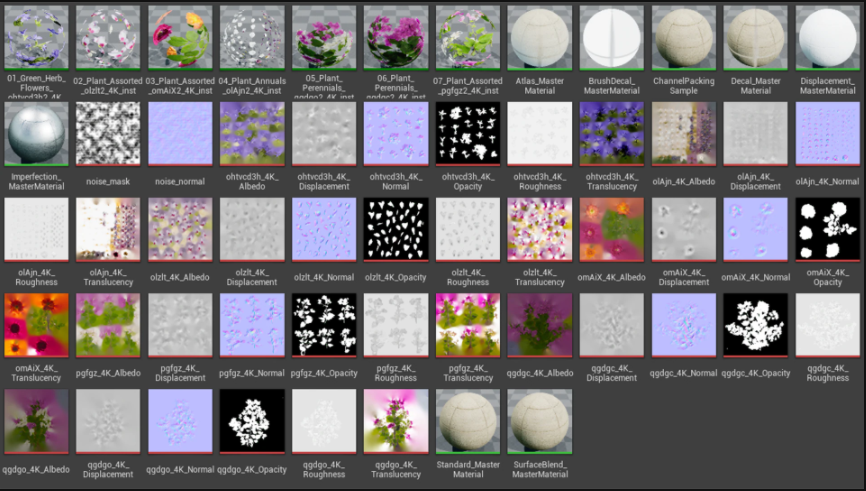
\includegraphics[width=.7\linewidth]{flower1.png}
		\caption{Çiçekler}\label{Fig:Data7}
		\end{minipage}\hfill
		\begin{minipage}{0.48\textwidth}
			\centering
			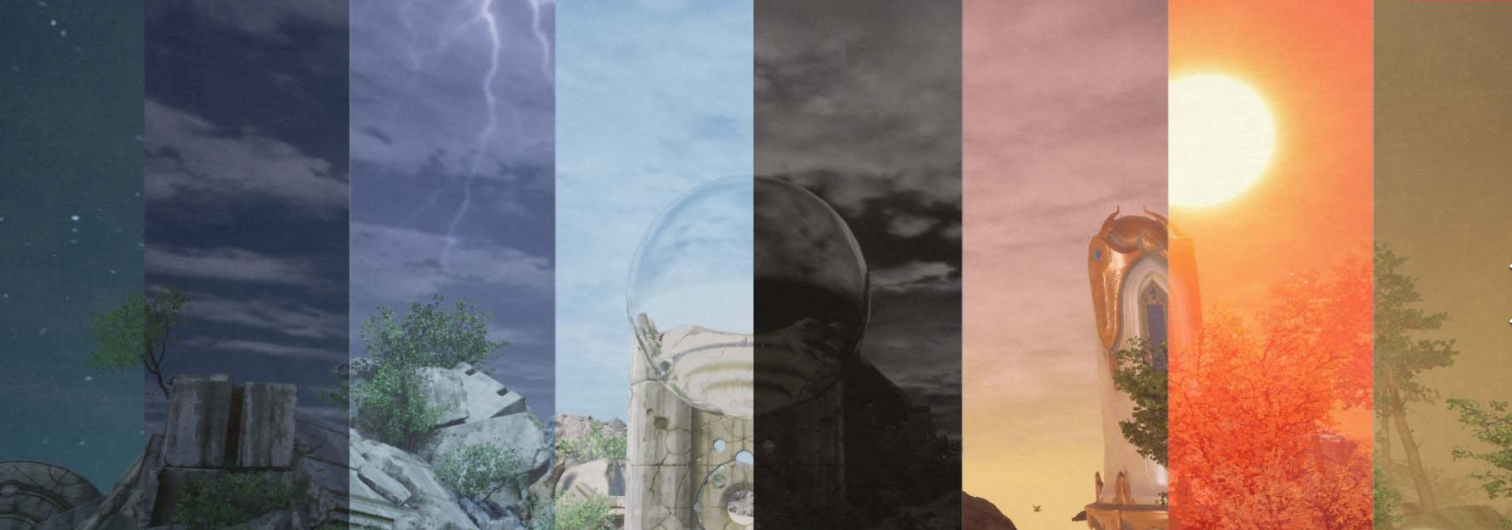
\includegraphics[width=.7\linewidth]{sky.png}
		\caption{Sky}\label{Fig:Data8}
		\end{minipage}
	\end{figure}
	
	\newpage
	\begin{landscape}
		\subsection{Sistem Tasarımı}
		\begin{figure}[!ht]%htbp
			\caption{GANTT CHART}
			\centering
			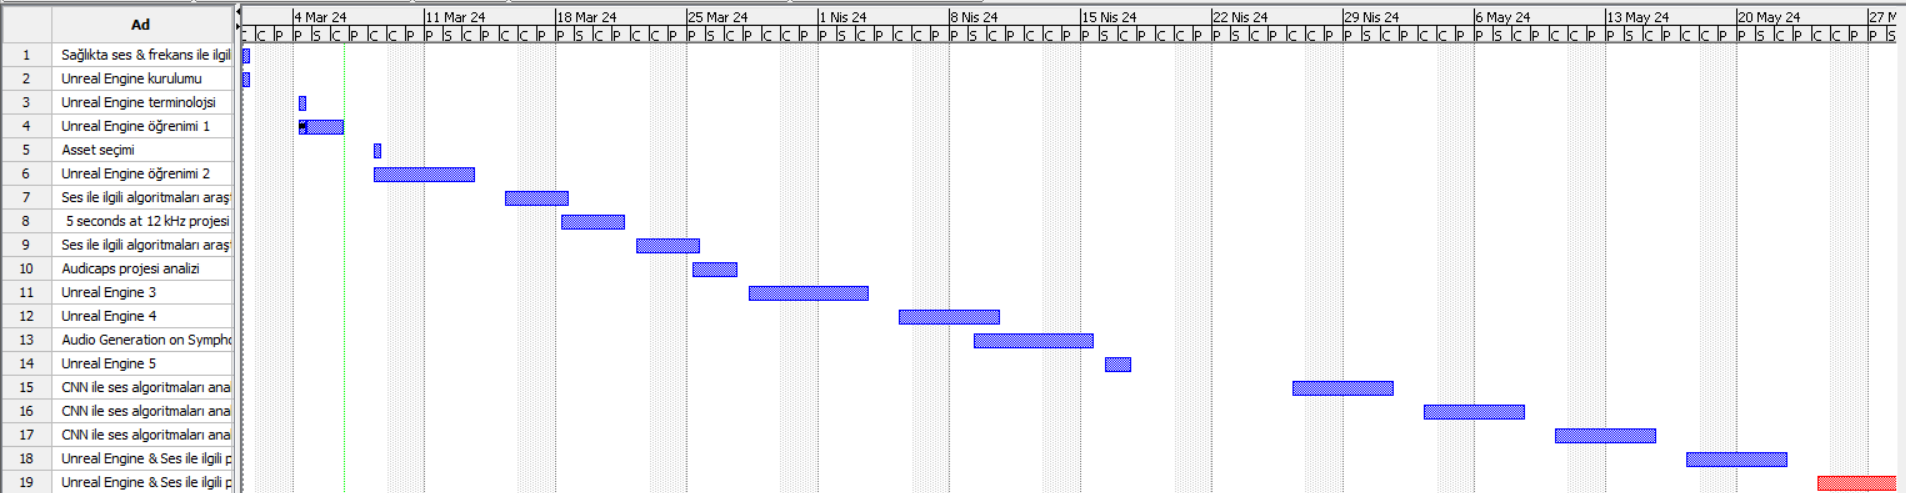
\includegraphics[height= 5 cm]{sound_gantt_chart1.png}
			\label{gantt}
		\end{figure}
	\end{landscape}
	\newpage
	\section{Veriler - Frekans Değerleri}\vspace*{1\baselineskip}
	\begin{itemize}
		\item 40Hz  : Alzheimer hastalığının terapi yöntemleri olarak nöral yanıtı uyarmak veya demans semptomlarını azaltmak için 40Hz titreşimli ses ve 810 nanometre ışık frekansı kullanılarak gama beyin dalgalarıyla hafızanın uyarılmasına sağlanmıştır. 
		
		\item 174Hz : Hem ağrının hem de stresin azaltılması ile ilişkili olan 174Hz, alternatif tıpta insan sağlığı üzerinde farklı olumlu etkilere sahip olduğuna inanılan kutsal müzikte kullanılan bir dizi ton olan Solfeggio frekanslarından biridir.
		
		\item 285Hz : Kesiklerin, yanıkların ve diğer fiziksel yaraların iyileşmesinde etkili olan 285 hertz ses frekansının vücutta hücresel rejenerasyonu aktive etmesi ve bir yaralanma durumunda kendini iyileştirmesi için teşvik etmesi beklenir. Ayrıca Solfeggio frekanslarından biridir.
		
		\item 396Hz : Korkunun ve diğer olumsuz duyguların giderilmesi ile ilişkili olan bu frekans Solfeggio frekanslarından da biridir. Suçluluk duygusunu yenmek amacıyla manevi müziğe etkili bir katkı sağlar. 396 hertz frekansları kök çakrayı dengelerken, aynı zamanda keder gibi olumsuz duyguları; olumlu, neşeli gibi duygulara dönüştürür. 
		
		\item 417Hz : Fiziksel rahatsızlıklara odaklanmak yerine, 417 hz (Solfeggio frekanslarından bir diğeri) içeren iyileştirici ses terapisi, geçmiş bir travmayı çevreleyen enerji veya ortamdaki negatif enerjiler gibi negatif enerjinin giderilmesine odaklanır. 417 hertz terapisi duygusal blokajları çözmek ve sakral çakrayı aktive etmek için tasarlanmıştır. 
		
		\item 432Hz : 432 hertz terapisi kalp çakrasını hedefler ve 432 hertz frekansını dinlemenin daha yüksek düzeyde zihinsel ve duygusal berraklığa yol açması beklenir. 432 hertz ayarının opera şarkıcılarını ayarlamak için en uygun olduğu düşünülür ve daha yüksek bir ruhsal gelişim seviyesiyle ilişkilendirilir.
		
		\item 440Hz : 440 hertz ile 432 hertz arasında ayarlanan müzik, dinleyicinin bilişsel gelişimine yardımcı olan "serebral" müzik olarak kabul edilir. 440 hertz'deki ses frekanslarının üçüncü göz çakrasını aktive ettiği kabul edilir.
		
		\item 528Hz : Aşk frekansı olarak da bilinen 528 hertz, Solfeggio frekanslarının en bilinen ve popüler olanlarından biridir. Bu müzik tonu aynı zamanda "mucize notası" olarak da bilinir ve yazılı tarih öncesinden beri yerli halklarda bereketle ilişkili bir ses olarak kullanılmıştır. 
		
		\item 639Hz : 639 hertz kalp çakrasını etkileyen bir ses frekansıdır. Bu ses frekansı, olumlu duygular üretmeyi ve uyumlu kişiler arası ilişkilere daha fazla uyum sağlamayı amaçlayan terapiyle ilişkilidir. Terapi olarak, 639 hertz maruziyeti daha net iletişim uygulamalarını ve durumsal farkındalığı teşvik eder.
		
		\item 852Hz : Zihni aşırı düşünmekten, müdahaleci düşüncelerden ve olumsuz düşünce kalıplarından uzaklaştırmakla ilişkilendirilen bir tondur. Düşüncesel yoğunluğun fazla olduğu depresyon ve anksiyete süreçlerini iyileştirmeyi hızlandırmak adına kullanılmaktadır. Bu ses frekansına maruz kalmak, olumsuz düşüncelerin bu psikolojik rahatsızlıklardaki rolünü hafifletmeye yardımcı olabilir.
		
		\item 963Hz : 963 hertz ses frekansları epifiz bezinin aktivasyonu ve yüksek ruhsal gelişim ile ilişkilidir. 963 hertz frekansı hem "saf mucize tonu" hem de "tanrıların frekansı" olarak bilinir. 963 taç çakranın aktivasyonu ve tüm insanlığın kaynağına bağlantı ile ilişkilidir.
	\end{itemize}	
	
	Gördüğünüz gibi, hem psikiyatrik hastalıklarla ilişkili bilişsel düşünce süreçlerini değiştirmek hem de bir hastalığa karşı koymak için fiziksel iyileştirici etkiler üretmek için iyileştirici bir uygulamada kullanılabilecek birçok farklı ses frekansı vardır\cite{benefits}. 
	
	\section{Beklenen Sonuçlar}
	Proje sonucu, farklı frekans aralıklarındaki seslerin insan vücudu üzerindeki fizyolojik ve psikolojik etkileri deneyimlenilebilinen ortamı hazırlamaktır. 
	Ayrıca yapay zeka ile ses üretimine odaklanan bu proje, günümüzdeki yaşanılan problemlerin sonucundaki olumsuz duyguları, iyileştirici etkiye sahip farklı frekanslardaki sesleri kullanarak olumsuz duygularını azaltarak, iyileştirme ve motivasyon sağlama yönünde hayatlarını desteklemektir.	\newline
	
	
	Frekansların iyileştirici etkisini desteklemek amacıyla unreal engine ortamındaki sanal gerçeklik teknolojisi ile  aynı zamanda insanı huzurlu hissettiren ortamlarda bu deneyimi sağlayarak rahatlama, stres azaltma ve motivasyon gibi durumları destekleyerek zihinsel iyileşmeyi amaçlamaktadır.
	\newpage
	\bibliographystyle{ieeetr}
	\bibliography{references}
	
\end{document}